\chapter{補題1の検証}
本章では、\ref{hypothesis}節で定義した補題1を検証する。

\section{補題1}
\firstLemma
% 成員の行動を観察できない外部の強制執行力が存在すると仮定した上で、
% 完全に合理的な成員達に 合意された約束を履行させるインセンティブ設計は不可能である。

\section{検証方法}
成員の行動を観察できない外部の強制執行力として「評判システム」(\ref{reputationSystem}節)の存在を仮定し、
2人の成員が、そのシステムを用いて約束を交わす「約束・評判ゲーム」(\ref{promiseReputationGame})について考える。
このとき、各成員が約束によって生じる価値と「評判スコア」の合計を最大化しようとする場合、
約束が履行されるような「評判スコア」の組を「評判システム」から決定できないことを示す。

% \begin{description}
%   \item[仮定1] 報告者は約諾者が約束を履行したか観察できる。
%   \item[仮定2] 報告者以外の成員は約諾者が約束を履行したか観察できない。 
%   \item[仮定3] 「評判システム」は約諾者が約束を履行したか観察できない。
% \end{description}

\section{評判システム}
\label{reputationSystem}
「評判システム」とは、初期の各成員の「評判スコア」と報告された約束の記録に基づいて、各成員の「評判スコア」を決定するシステムである。
約束の記録とは、約諾者が約束を履行したかについての情報であり、約諾者、報告者、結果(「履行」か「反故」)からなる。
このシステムから成員の行動を観察することはできないため、約諾者が真に約束を履行したか否かと報告された結果が同じとは限らない。
このシステムは、「約束・評判ゲーム」(\ref{promiseReputationGame}節)において、強制執行力としての役割を果たす。

% \subsection{約束の記録}

\section{約束・評判ゲーム}
\label{promiseReputationGame}
「約束・評判ゲーム」とは、約諾者($promisor$)と報告者($reporter$)の2人によって行われるゲームである。
約諾者は2者間で合意された約束を履行する、もしくは反故にする。
それに対して報告者は約束の結果(「履行」か「反故」)を決定し、約束の記録を「評判システム」に報告する。

\begin{description}
  % \centering
  \item[step1]  $promisor$は合意された約束を履行する、もしくは反故にする.
  \item[step2]  $reporter$は「履行」か「反故」を「評判システム」に報告する.
\end{description}


\subsection{展開型ゲーム}
\label{prgame-by-extensive-form}

これは図\ref{prgametree}のゲームの木のような展開型ゲームとして表せる.
各変数については下記の通りである。

\textbf{step1}で$promisor$が約束を履行するか反故にするかと、
\textbf{step2}で$reporter$が「履行」を報告するか「反故」を報告するかで4つの結果がある。
また,「評判システム」からは$promisor$と$reporter$の行動を観察できないため,
\textbf{step2}での$reporter$の報告に基づいて$promisor$と$reporter$の「評判スコア」が決定しなければならない.
それ故、①と③,②と④はそれぞれ$c_k$($k$は任意の添字)を除いて同じ利得でなくてはならない.
また、$promiser$にとっては約束を履行することによって生じる効用は約束を反故にすることによって生じる効用より小さく($c_{p1} < c_{p2}$)、
$reporter$にとっては約束が履行されることによって生じる効用は約束が反故にされることによって生じる効用より大きい($c_{r1} > c_{r2}$)ものとする。

\subsubsection{各変数の定義}
\label{prgamePayoffVariables}
\begin{description}
  % \centering
  \item[$c_{p1}$]… 約束が履行された場合の$promisor$の「評判スコア」の変化量以外の効用
  \item[$c_{p2}$]… 約束が反故にされた場合の$promisor$の「評判スコア」の変化量以外の効用
  \item[$c_{r1}$]… 約束が履行された場合の$reporter$の「評判スコア」の変化量以外の効用
  \item[$c_{r2}$]… 約束が反故にされた場合の$reporter$の「評判スコア」の変化量以外の効用
  \item[$r_{ps}$]… 「履行」が報告された場合の$promisor$の「評判スコア」の変化量
  \item[$r_{pf}$]… 「反故」が報告された場合の$promisor$の「評判スコア」の変化量
  \item[$r_{rs}$]… 「履行」が報告された場合の$reporter$の「評判スコア」の変化量
  \item[$r_{rf}$]… 「反故」が報告された場合の$reporter$の「評判スコア」の変化量
\end{description}

\begin{figure*}
  \centering
  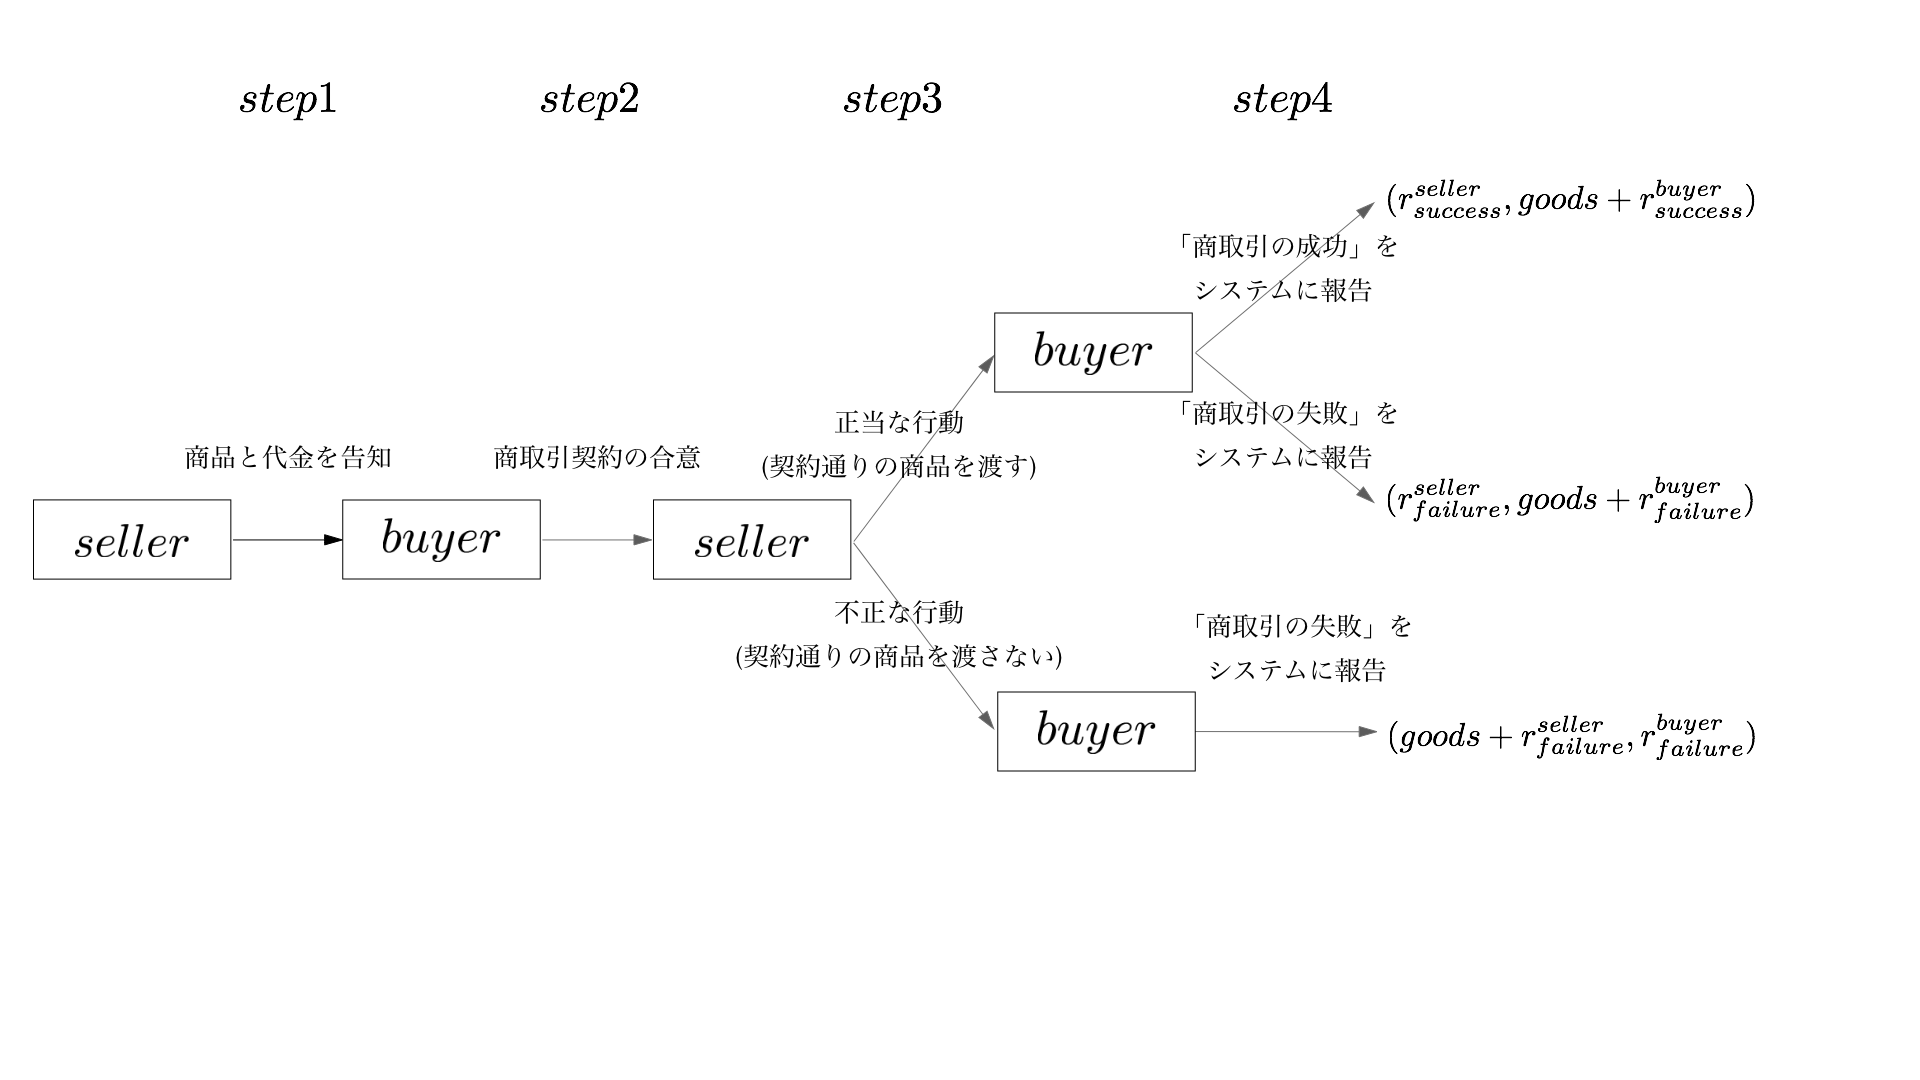
\includegraphics[width=1\linewidth]{./06_ethical-prgame/ethical-gametree.png}
  \caption{「告発する約束・評判ゲーム」のゲーム木}
  \label{ethical-gametree}
\end{figure*}

\subsection{各プレイヤーの戦略}
\label{playersStrategy}
この展開型ゲームにおける$promisor$と$reporter$の行動は、下記のような戦略として表せる。

\subsubsection{$promisor$の戦略}
\begin{description}
  \item[$s_{p1}$]… 約束を履行する
  \item[$s_{p2}$]… 約束を反故にする
\end{description}

\subsubsection{$reporter$の戦略}
\begin{description}
  \item[$s_{r1}$]… $promisor$が約束を履行した場合は「履行」,反故にした場合は「反故」を報告する
  \item[$s_{r2}$]… $promisor$が約束を履行した場合は「履行」,反故にした場合は「履行」を報告する
  \item[$s_{r3}$]… $promisor$が約束を履行した場合は「反故」,反故にした場合は「反故」を報告する
  \item[$s_{r4}$]… $promisor$が約束を履行した場合は「反故」,反故にした場合は「履行」を報告する
\end{description}

\subsection{非協力戦略型ゲーム}
これらの戦略を用いて、先に述べた展開型ゲームは表\ref{prgametable}のような非協力戦略型ゲームとして書き換えられる.

% Success Reported on True Success
\newcommand{\SROS}{ $(c_{p1} + r_{ps},$ \\$c_{r1} + r_{rs})$ }
\newcommand{\FROF}{ $(c_{p2} + r_{ps},$ \\$c_{r2} + r_{rs})$ }
\newcommand{\FROS}{ $(c_{p1} + r_{pf},$ \\$c_{r1} + r_{rf})$ }
\newcommand{\SROF}{ $(c_{p2} + r_{pf},$ \\$c_{r2} + r_{rf})$ }
\newcommand{\tabularc}[1]{\begin{tabular}{c} #1 \end{tabular}}

\begin{table*}[h]
  \begin{tabular}{|l|l|l|l|l|l|}
  \hline
  \multicolumn{2}{|l|}{\multirow{2}{*}{}} & \multicolumn{4}{l|}{$Reporter$} \\ \cline{3-6}
  \multicolumn{2}{|l|}{}                  &$s_{r1}$&$s_{r2}$&$s_{r3}$&$s_{r4}$\\ \hline
  \multirow{2}{*}{$Promisor$}
  &$s_{p1}$&\tabularc{\SROS}&\tabularc{\SROS}&\tabularc{\FROS}&\tabularc{\FROS}\\ \cline{2-6}
  &$s_{p2}$&\tabularc{\SROF}&\tabularc{\FROF}&\tabularc{\SROF}&\tabularc{\FROF}\\ \hline
  \end{tabular}
  \caption{「約束・評判ゲーム」の利得票表}
  \label{prgametable}
\end{table*}

\section{不正が防止される条件}
表\ref{prgametable}より,「約束・評判ゲーム」において、約束が履行されるためには、
$promisor$と$reporter$のとる戦略組が$ (s_{p1}, s_{r1})$、$(s_{p1}, s_{r2})$, $(s_{p1}, s_{r2})$, $(s_{p1}, s_{r2})$のいずれかになる必要がある.
各プレイヤーが戦略$s$をとったときの利得を$R$とし、その期待値を$E(R|s)$とする。
全てのプレイヤーが完全に合理的な場合、$(s_{p1}, s_{r1})$か$(s_{p1}, s_{r2})$のいづれかの戦略組に帰着させるためには,

\begin{description}
  \centering
  \item[条件①] $E(R|s_{p1})>E(R|s_{p2})$かつ$E(R|s_{r1})>\max\{E(R|s_{r2}), E(R|s_{r3}), E(R|s_{r4}) \}$
  \item[条件②] $E(R|s_{p1})>E(R|s_{p2})$かつ$E(R|s_{r2})>\max\{E(R|s_{r1}), E(R|s_{r3}), E(R|s_{r4}) \}$
  \item[条件③] $E(R|s_{p1})>E(R|s_{p2})$かつ$E(R|s_{r3})>\max\{E(R|s_{r1}), E(R|s_{r2}), E(R|s_{r4}) \}$
  \item[条件④] $E(R|s_{p1})>E(R|s_{p2})$かつ$E(R|s_{r4})>\max\{E(R|s_{r1}), E(R|s_{r2}), E(R|s_{r3}) \}$
\end{description}

のいづれかを満たす$(r_{ps}, r_{pf}, r_{rs}, r_{rf})$の組を「評判システム」から決定できる必要がある.
本章ではこれが不可能であることを示す.

\section{命題}
条件①〜④のいづれかを満たす$(r_{ps}, r_{pf}, r_{rs}, r_{rf})$の組を「評判システム」から決定することはできない.
  
\section{証明}
\label{verification1}
各プレイヤーが戦略$s_{k}$をとる確率を$p_{k}$とする.

\begin{gather}
  0 \leq p_{k} \leq 1 \nonumber \\
  p_{p1} + p_{p2} = 1 \nonumber \\
  p_{r1} + p_{r2} + p_{r3} + p_{r4} = 1 \label{condition1}
\end{gather}

\subsubsection{各戦略の期待利得}
$promisor$と$reporter$の各戦略の期待利得は次のように表せる.
\begin{eqnarray}
  E(R|s_{p1}) &=& p_{r1} (c_{p1} + r_{ps}) + p_{r2} (c_{p1} + r_{ps}) + p_{r3} (c_{p1} + r_{pf}) + p_{r4} (c_{p1} + r_{pf}) \nonumber \\
              &=& c_{p1} + p_{r1} r_{ps} + p_{r2} r_{ps} + p_{r3} r_{pf} + p_{r4} r_{pf} \because\eqref{condition1} \label{expectedA} \\
  E(R|s_{p2}) &=& p_{r1} (c_{p2} + r_{pf}) + p_{r2} (c_{p2} + r_{ps}) + p_{r3} (c_{p2} + r_{pf} ) + p_{r4} (c_{p2} + r_{ps}) \nonumber \\
              &=& c_{p2} + p_{r1} r_{pf} + p_{r2} r_{ps} + p_{r3} r_{pf} + p_{r4} r_{ps} \because\eqref{condition1} \label{expectedB} \\
  E(R|s_{r1}) &=& p_{p1} (c_{r1} + r_{rs}) + p_{p2} (c_{r2} + r_{rf}) \label{expectedR1} \\
  E(R|s_{r2}) &=& p_{p1} (c_{r1} + r_{rs}) + p_{p2} (c_{r2} + r_{rs}) \label{expectedR2} \\
  E(R|s_{r3}) &=& p_{p1} (c_{r1} + r_{rf}) + p_{p2} (c_{r2} + r_{rf}) \label{expectedR3} \\
  E(R|s_{r4}) &=& p_{p1} (c_{r1} + r_{rf}) + p_{p2} (c_{r2} + r_{rs}) \label{expectedR4} \nonumber
\end{eqnarray}

\subsubsection{条件①が成り立たないことの証明}

条件①が成り立たないことを示すために、その必要条件である下記の2つの条件について考える。

\begin{gather}
  E(R|s_{r1}) > E(R|s_{r2}) \label{conditionA} \\
  E(R|s_{r1}) > E(R|s_{r3}) \label{conditionB}
\end{gather}

\eqref{conditionA}を満たすためには、
\begin{eqnarray*}
  &&E(R|s_{r1}) > E(R|s_{r2}) \\
  &\therefore& p_{p1} (c_{r1} + r_{rs}) + p_{p2} (c_{r2} + r_{rf}) > p_{p1} (c_{r1} + r_{rs}) + p_{p2} (c_{r2} + r_{rs}) \because\eqref{expectedR1}\eqref{expectedR2}  \\
  &\therefore& p_{p2} r_{rf} - p_{p2} r_{rs} > 0 \\
  &\therefore& p_{p2} (r_{rf} - r_{rs}) > 0 \\
\end{eqnarray*}

つまり、

\begin{equation}
  p_{p2} > 0 \nonumber
\end{equation}

かつ

\begin{equation}
\label{quad1}
  0 > r_{rs} - r_{rf}
\end{equation}

を満たす必要がある。\\


\eqref{conditionB}を満たすためには、
\begin{eqnarray*}
  &&E(R|s_{r1}) > E(R|s_{r3}) \\
  &\therefore& p_{p1} (c_{r1} + r_{rs}) + p_{p2} (c_{r2} + r_{rf}) > c_{p2} + p_{r1} r_{pf} + p_{r2} r_{ps} + p_{r3} r_{pf} + p_{r4} r_{ps}) \because\eqref{expectedR1}\eqref{expectedR3}\\
  &\therefore& p_{p1} r_{rs} + p_{p2} r_{rf} > p_{p1} r_{rf} + p_{p2} r_{rf} \\
  &\therefore& p_{p1} (r_{rs} - r_{rf}) > 0
\end{eqnarray*}

つまり,

\begin{equation}
   p_{p1} > 0 \nonumber
\end{equation}

かつ

\begin{equation}
   \label{quad2}
   r_{rs} - r_{rf} > 0
\end{equation}

を満たす必要がある。\\

ここで(\ref{quad1})と(\ref{quad2})を同時に満たすことはできないため,条件①は成り立たない.\\

\subsubsection{条件④が成り立たないことの証明}
また、同様に条件④も成り立たない。

\subsubsection{条件②が成り立たないことの証明}
次に、条件②の必要条件である

\begin{gather}
  E(R |s_{p1}) > E(R |s_{p2}) \label{conditionC}
\end{gather}

について考える。\\

\eqref{conditionC}を満たすためには,
\begin{eqnarray*}
  &&E(R |s_{p1}) > E(R |s_{p2}) \\
  &\therefore& c_{p1} + p_{r1} r_{ps} + p_{r2} r_{ps} + p_{r3} r_{pf} + p_{r4} r_{pf} > c_{p2} + p_{r1} r_{pf} + p_{r2} r_{ps} + p_{r3} r_{pf} + p_{r4} r_{ps} \\
  &\therefore& c_{p1} + p_{r1} r_{ps} + p_{r4} r_{pf} > c_{p2} + p_{r1} r_{pf} + p_{r4} r_{ps} \\
  &\therefore& c_{p1} - c_{p2} + p_{r1} r_{ps} + p_{r4} r_{pf} + p_{r1} r_{pf} - p_{r4} r_{ps} > 0 \\
  &\therefore& p_{r1}(r_{ps} - r_{pf}) - p_{r4}(r_{ps} - r_{pf}) + c_{p1} - c_{p2} > 0 \\
  &\therefore& (p_{r1} - p_{r4})(r_{ps} - r_{pf}) + c_{p1} - c_{p2} > 0 \\
  &\therefore& (p_{r1} - p_{r4})(r_{ps} - r_{pf} + \frac{ c_{p1} - c_{p2} }{p_{r1} - p_{r4}}) > 0
\end{eqnarray*}

を満たす必要がある.つまり,\\

$p_{r1} > p_{r4}$のとき, 
\begin{eqnarray}
  &&r_{ps} - r_{pf} + \frac{ c_{p1} - c_{p2} }{p_{r1} - p_{r4}} > 0\nonumber \\
  &\therefore&r_{ps} - r_{pf} > \frac{ c_{p2} - c_{p1} }{ p_{r1} - p_{r4} } \nonumber
\end{eqnarray}

$p_{r1} < p_{r4}$のとき, 
\begin{eqnarray}
  &&r_{ps} - r_{pf} + \frac{ c_{p1} - c_{p2} }{p_{r1} - p_{r4}} < 0 \nonumber \\
  &\therefore&r_{ps} - r_{pf} < \frac{ c_{p2} - c_{p1} }{ p_{r1} - p_{r4} } \nonumber
\end{eqnarray}

を満たせばよい.\\

ここで、$E(R|s_{r2})>\max\{E(R|s_{r1}), E(R|s_{r3}), E(R|s_{r4}) \}$が成り立つと仮定する。\\

このとき全ての合理的なプレイヤーは戦略$s_r2$をとり必ず「履行」を報告するため、
「評判システム」から$p_{r1}$と$p_{r4}$を推定することはできない。\\

ゆえに、「評判システム」から条件②を満たすような$(r_{ps}, r_{pf})$の組を決定できない.\\

\subsubsection{条件③が成り立たないことの証明}
また、同様に条件③も成り立たない。

以上より,条件①と条件②のいづれかを満たす
$(r_{ps}, r_{pf},r_{rs},r_{rf})$の組を「評判システム」から決定することはできない.\\

Q.E.D. \\